\documentclass[../proyecto.tex]{memoir}

\begin{document}

\chapter{Análisis}

Las estimaciones de los métodos Monte Carlo dependen en gran medida de la anchura del intervalo de confianza $[\mu+3\sigma, \mu-3\sigma]$. Dicha anchura se reduce con el incremento del número de muestras aleatorias pero lo hace lentamente con el consecuente incremento de tiempo de computación. Por esta razón se crean métodos alternativos conocidos como métodos de reducción de la varianza. En esta sección introducimos uno que se adecúa a nuestro problema y que utilizaremos en las todas las ejecuciones posteriores.

\section{Reducción de la varianza}

En la \autoref{fig:3-1} visualizamos la evolución del área del cuadrado más pequeño que contiene a todas las células en cada iteración de juego de vida. Para el contenido de esta sección no es relevante la configuración inicial de la que se han obtenido los datos. Cada punto representa una estimación Monte Carlo, para los puntos de color naranja no se puede rechazar la hipótesis nula de que sigan un distribución normal, los de color azul sí rechazan la hipótesis nula y por tanto no podemos afirmar nada acerca de su intervalo de confianza.

El intervalo de confianza $[\mu+3\sigma, \mu-3\sigma]$ crece a medida que la iteración se aleja de la configuración inicial, de decir, la varianza aumenta. Es posible reducirla aumentando el número de simulaciones globalmente e incrementando notablemente el tiempo de cálculo. Sin embargo para el número prefijado de simulaciones se obtienen intervalos de confianza lo suficientemente pequeños en las iteraciones iniciales, por tanto proponemos incrementar el número de simulaciones a medida que las iteraciones aumenten. Este incremento requiere de la adición de nuevas simulaciones en cada iteración, las cuales serán escogidas aleatoriamente de las ya existentes modificando la semilla para no obtener simulaciones duplicadas. Experimentalmente hemos observado que un valor que muestra buenos resultados sin aumentar excesivamente el tiempo de cálculo es un incremento en cada iteración de una décima parte del valor inicial de simulaciones. Finalmente es posible observar la reducción del intervalo de confianza que conlleva dicho incremento en la \autoref{fig:3-2}.

\begin{figure}[H]
	\centering
    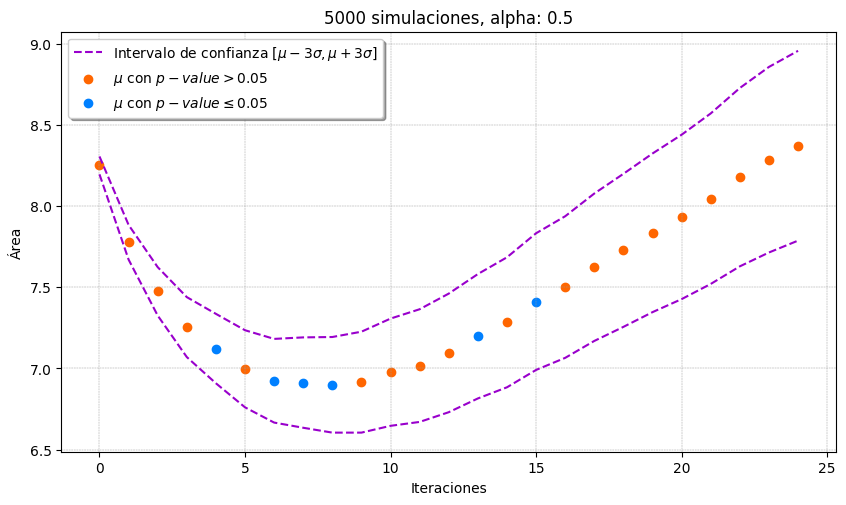
\includegraphics[width=\textwidth]{./images/iteracion_without_inc.png}
    \caption{Ejecución sin incremento del valor inicial de simulaciones cada iteración.}
    \label{fig:3-1}
\end{figure}

\begin{figure}[H]
        \centering
        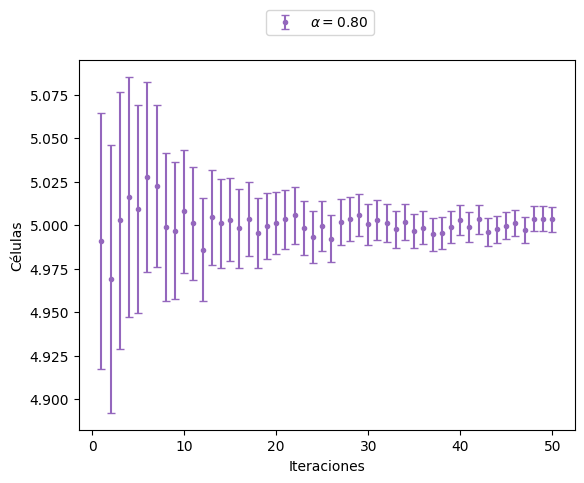
\includegraphics[width=\textwidth]{./images/iteracion_inc.png}
        \caption{Ejecución con incremento del 10\% del valor inicial de simulaciones en cada iteración.}
        \label{fig:3-2}
\end{figure} 

%\section{Efecto de la variación de la distribución de probabilidad}

%En esta sección vamos a estudiar el efecto de la generación de números aleatorios para las simulaciones utilizando distribuciones de probabilidad distintas a la uniforme. Nos resulta de especial interés algún tipo de distribución que este relacionada con el valor de $\alpha$-asincronicidad que empleemos. Una buena candidata es la distribución normal con media $\mu=\alpha$

%Cuidado, una normal centrada el $\alpha$ no da valores entre 0 y 1, hay que hacer alguna magia más


\end{document}